\documentclass{article}

\usepackage{graphicx}
\usepackage{authblk}
\usepackage{url}
\usepackage[german]{babel}
\usepackage{csquotes}
\usepackage{wrapfig}
\usepackage[sorting=none]{biblatex}
\usepackage{listings}
\usepackage{hyperref}
\usepackage{dirtree}
\usepackage{upquote}
\usepackage[edges]{forest}
\definecolor{folderbg}{RGB}{124,166,198}
\definecolor{folderborder}{RGB}{110,144,169}
\newlength\Size
\setlength\Size{4pt}

\tikzset{%
  folder/.pic={%
    \filldraw [draw=folderborder, top color=folderbg!50, bottom color=folderbg] (-1.05*\Size,0.2\Size+5pt) rectangle ++(.75*\Size,-0.2\Size-5pt);
    \filldraw [draw=folderborder, top color=folderbg!50, bottom color=folderbg] (-1.15*\Size,-\Size) rectangle (1.15*\Size,\Size);
  },
  file/.pic={%
    \filldraw [draw=folderborder, top color=folderbg!5, bottom color=folderbg!10] (-\Size,.4*\Size+5pt) coordinate (a) |- (\Size,-1.2*\Size) coordinate (b) -- ++(0,1.6*\Size) coordinate (c) -- ++(-5pt,5pt) coordinate (d) -- cycle (d) |- (c) ;
  },
}
\forestset{%
  declare autowrapped toks={pic me}{},
  pic dir tree/.style={%
    for tree={%
      folder,
      font=\ttfamily,
      grow'=0,
    },
    before typesetting nodes={%
      for tree={%
        edge label+/.option={pic me},
      },
    },
  },
  pic me set/.code n args=2{%
    \forestset{%
      #1/.style={%
        inner xsep=2\Size,
        pic me={pic {#2}},
      }
    }
  },
  pic me set={directory}{folder},
  pic me set={file}{file},
}

\addbibresource{references.bib}

\graphicspath{ {./img/} }

\newcommand\blankpage{%
    \null
    \thispagestyle{empty}%
    \newpage}
    
\newcommand{\dateline}[3]{%
\par\medskip\noindent
\makebox[\textwidth][s]{\rlap{#1}\hfill#2\hfill\llap{#3}}%
\par\medskip}

\author[1]{Tobias Nöthlich}
\author[1]{Florian Richter}
\author[1]{Tim Krieg}

\title{Implementierung einer Testsuite, zur Untersuchung von Möglichkeiten für DoS-Angriffe auf DTN-Protokollimplementierungen}





\begin{document}

\pagenumbering{arabic}


\begin{titlepage}

\begin{figure}[h]
\begin{flushleft}

\includegraphics[trim= 0 0 0 0 , clip, width=6cm]{img/logo.eps} 
\end{flushleft}
\end{figure}
\noindent
Fakultät Informatik\\
Institut für Systemarchitektur, Lehrstuhl Rechnernetze \\

\begin{center}
\Huge
\textbf{Implementierung einer Testsuite, zur Untersuchung von Möglichkeiten für DoS-Angriffe auf DTN-Protokollimplementierungen} \\
\normalsize
\vspace{1cm}

\end{center}

\vspace{1cm}
\noindent
\textbf{\large{Tobias Nöthlich}} \\
\textbf{\large{Florian Richter}} \\
\textbf{\large{Tim Krieg}} \\

\vspace{1cm}
\noindent
{\LARGE Projektdokumentation} \\

\vspace{1cm}
\noindent
Betreuer\\
\textbf{\large{Dr.-Ing. Marius Feldman}} \\

\vspace{1cm}
\dateline{Wintersemester 2020/2021}{}{Abgabe: 05. Februar 2021}
\end{titlepage}

\tableofcontents

\newpage

\section{Einleitung}

Die Kommunikation in Katastrophengebieten oder besonders im interplanetaren Raum ist aufgrund von großen Entfernungen und vermehrtem Datenverlust stark erschwert, sodass gewöhnliche Internetverbindungen keine verlässliche Lösung bieten. Um in diesen Situationen trotzdem stabile Verbindungen zu gewährleisten, wird z. B. von der NASA Delay/Disruption Tolerant Networking (DTN) verwendet.
DTN-Protokolle sind speziell für Verbindungen mit langer oder variabler Verzögerung, asymmetrischen Datenraten und vielen Disruptionen konzipiert. Diese funktionieren, in dem sie durch Store-and-Forwarding, Bundles von einem Knoten (engl. Node) zum Nächsten schicken. Bei Unterbrechung der Verbindung werden die Bundles bei den Nodes zwischengespeichert. Dadurch können Daten inkrementell entlang eines Pfades zum Ziel gesendet werden und es wird keine durchgehende Verbindung wie bei TCP benötigt. 
Die erschwerten Bedingungen in der Kommunikation und das Speichern auf Zwischenpunkten, sowie die bisher nicht entwickelten Sicherheitsmechanismen machen die Verbindung anfällig für unterschiedliche Denial-of-Service Attacken. Für die Untersuchung verschiedener solcher Attacken und deren Auswirkungen haben wir diese Testsuite entwickelt und so gestaltet, dass sie in Zukunft noch auf weitere Szenarien erweitert werden kann.  

\section{Anforderungen}
\begin{itemize}
    \item Das Toolkit soll auf Linux ausführbar sein.
    \item Es sollen verschiedene Szenarien mitgeliefert werden.
    \item Das Hinzufügen von weiteren Szenarien muss möglich sein.
    \item Es muss ein Setup beiliegen, um das Toolkit problemlos installieren zu können.
    \item Schreiben einer vollständigen Dokumentation.
\end{itemize}

\section{Implementation}
\subsection{Verzeichnisstruktur}
\subsubsection{Anwendungsverzeichnis (nach Setup)}\label{avz}
\begin{forest}
  pic dir tree,
  where level=0{}{% folder icons by default; override using file for file icons
    directory,
  },
  [dtn-dos
    [Documentation
      [img, label=right:Enthält die in der Dokumentation verwendeten Bilder.
      ]
      [Documentation\_dtndos.pdf, file, 
      ]
      [main.tex, file
      ]
      [readme.txt, file
      ]
      [references.bib, file
      ]
    ]
    [Scenarios,
      [ion, label=right:Verzeichnis wird beim Setup nach /home/user/.core/configs kopiert.
      [BundleFlooding
      ]
      [ConfigTakeOver
      ]
      [ConfigTakeOverSatellite
      ]
      [DDoS
      ]
      [Slowloris
      ]
      [TestScenario
      ]
      ]
    ]
    [ion-open-source-4.0.0
    ]
    [core
    ]
    [.gitignore, file
    ]
    [README.md, file
    ]
    [setup.sh, file
    ]
    [start\_dtndos.sh, file
    ]
    [test.rc, file
    ]
  ]
\end{forest}
\subsubsection{Szenarioverzeichnis}\label{svz}
\begin{forest}
  pic dir tree,
  where level=0{}{% folder icons by default; override using file for file icons
    directory,
  },
  [Szenario, label=right:Beispielhafter Aufbau eines Szenarios.
    [n1, label=right:Verzeichnis des Knotens n1
     [n1.ionconfig, file, label=right: ION-interne Konfigurationsdatei des Knotens n1.
     ]
     [n1.rc, file, label=right: Netzwerkkonfigurationsdatei des Knotens n1.
     ]
    ]
    [n2, label=right: Jeder Knoten benötigt ein seperates Verzeichnis.
    [n2.ionconfig, file
     ]
     [n2.rc, file
     ]
    ]
    [Szenario.imn, file, label=right: CORE-Projektdatei des Szenarios
     ]
     [bundlecount.sh (optional), file, label=right: Zeigt Anzahl der Bundles.
     ]
     [bundlewatch.sh (optional), file, label=right: Zählt Bundles auf jedem Knoten.
     ]
     [cleanup.sh (optional), file, label=right: Entfernt temporäre Logfiles.
     ]
     [nodeSetup.sh, file, label=right: Startet ION auf den CORE-Knoten.
     ]
     [othervis.sh (optional), file, label=right: Enthält sonstige Visualisierungen.
     ]
     [pingvis.sh (optional), file, label=right: Visualisiert Ping zwischen Knoten.
     ]
  ]
\end{forest}
\newpage
\subsection{Shell Skripte}
Unser Ziel war es, ein möglichst einfach zu bedienendes Toolkit zu erstellen, welches ohne großen Aufwand installiert werden kann. Deshalb besteht dtn-dos aus zwei, für den die Szenarien ausführenden Endnutzer, wichtigen Skripten.
\subsubsection{Setup}
Das Setup und die Installation aller benötigten Dependencies erfolgt mittels des Skriptes \texttt{setup.sh}. Durch dieses werden die folgenden Dinge heruntergeladen, installiert und konfiguriert:
\begin{itemize}
    \item \texttt{xterm} - benötigt für die Visualisierungen
    \item \texttt{ncat} - benötigt für die Szenarien 'Config Take Over' und 'Config Take Over Satellite'
    \item CORE + dependencies - benötigt zum Aufbau der virtuellen Netzwerke
    \item ION DTN \cite{ion} - die DTN-Implementation, welche in den Szenarien zum Einsatz kommt
\end{itemize}
Im Laufe des Setups wird CORE bereits einmal gestartet um benötigte Konfigurationsdateien anzulegen. Der Benutzer kann dieses Fenster nach Abschluss des Setups einfach schließen.\par
Wir haben dtn-dos nur für Ubuntu entwickelt und auf Ubuntu 20.0.4 LTS getestet.
\subsubsection{Start}
Man kann dtn-dos mit dem \texttt{start\_dtndos.sh} Skript starten. Die Auswahl des zu startenden Szenarios erfolgt dabei über die Konsole, eine Auflistung aller verfügbaren Szenarien wird ebenfalls über die Konsole ausgegeben.\par
Nach Auswahl eines Szenarios wird automatisch die entsprechende Konfiguration von CORE geladen und zugehörige Visualisierungsskripte gestartet (mehr zur Visualisierung im Abschnitt \textbf{\ref{visualisierung}}). Eine Auflistung aller momentan implementierten Szenarien folgt im nächsten Abschnitt.
\newpage
\section{Szenarien}
\subsection{Bundle Flooding}
Das erste Szenario ist die Simulation eines Bundle Flooding Angriffs auf ein Netzwerkelement, das als Verbindungsstück zwischen einem Satelliten und dem Mission Control Center fungiert. Die für die Simulation genutzte Netzwerktopologie besteht aus fünf Elementen, welche im Common Open Research Emulator durch den \textbf{Router} Knotentypen emuliert werden.\par
\begin{figure}[h]
\centering
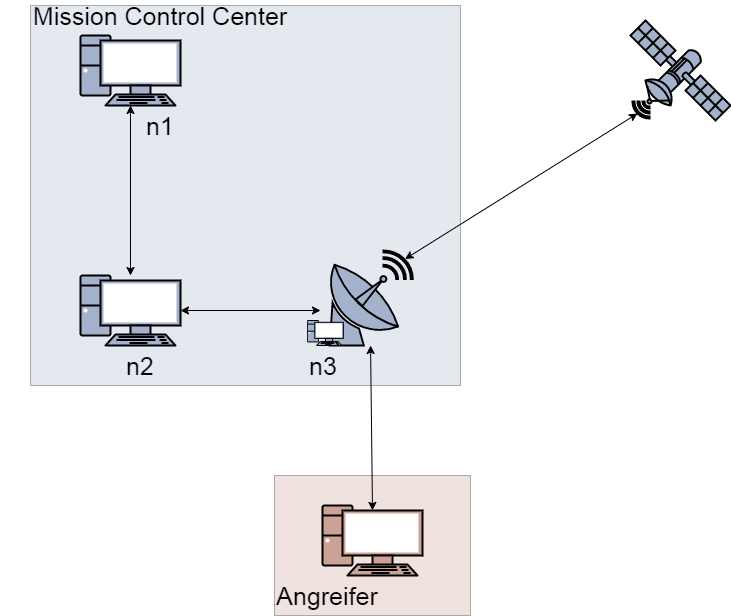
\includegraphics[width=0.5\textwidth]{flooding}
\caption{Netzwerktopologie des Bundle Flooding Szenarios. Die farbigen Boxen stehen dabei nicht für Netzwerkzugehörigkeit, sondern dienen nur der Veranschaulichung.}
\end{figure}
Das Grundprinzip des dem Szenario zugrunde liegenden Denial of Service Angriffs ist das Fluten des Zielsystems mit einer so großen Menge an Bundles, dass es nicht mehr in der Lage ist, den legitimen Traffic zuzustellen. Da Delay-Tolerant Networking Systeme (DTN-Systeme) insbesondere für Gebiete, in denen stabile Verbindungen nicht durchgehend möglich sind, konzipiert wurden, gibt es auch in diesem Szenario Verbindungsunterbrechungen zwischen Satellit und dem Mission Control Center. Da durch unterbrochene Verbindungen nicht zustellbare Bundles zunächst auf dem letzten erreichbaren Knoten gesichert werden, muss ein Angreifer lediglich einen Knoten mit instabiler Verbindung attackieren. Es ist allerdings von Nöten, dass der Angreifer Zugriff auf ein in das ION-Netz eingebundenes System hat, da ION die verfügbaren Kontakte aus einer Konfigurationsdatei liest. Es ist also nicht möglich, von außerhalb eine Verbindung zu einem bestehenden Netzwerk herzustellen.\par
Konkret auf unser Szenario bezogen, bedeutet dies, dass der \textit{Angreifer} ein System im Netzwerk übernommen hat und nun eine Verbindung zu \textit{n3} besteht. Er wird nun diesen Knoten mit an den \textit{Satelliten} adressierten Bundles fluten, bis  der restliche Netzwerkverkehr zum Erliegen kommt. Dabei reichen 50 Bundles pro Sekunde aus, um in kurzer Zeit die Übertragungskapazität der Leitung zwischen \textit{n3} und dem \textit{Satelliten} so zu beeinträchtigen, dass nur knapp ein Drittel der ursprünglichen Leistung für den restlichen Traffic zur Verfügung steht. Dies zeigt sich an den Round Trip Times (RTT) der Kommunikation zwischen \textit{n1} und dem \textit{Satelliten}. Hat ein Bundle Ping von \textit{n1} zum \textit{Satelliten} vor dem Start des DoS-Angriffs eine RTT von knapp einer Sekunde, so beträgt diese wenige Sekunden nach Start des DoS-Angriffs bereits über drei Sekunden. Circa fünf Sekunden nachdem der \textit{Angreifer} beginnt \textit{n3} zu fluten, ist ein Ping von \textit{n1} zum \textit{Satelliten} nicht mehr möglich, da bereits über 100 Bundles vom \textit{Angreifer} auf dem Knoten \textit{n3} auf die Weiterleitung zum \textit{Satelliten} warten.\par
Ein wichtiger Faktor zum Erfolg dieses Angriffes ist die von ION gegebene Möglichkeit, die Priorität der vom Bundle Ping ausgesendeten Bundles zu ändern. Durch das Versenden von Bundles mit der höchsten Priorität ist es dem \textit{Angreifer} möglich, die von ihm gesendeten Bundles an den Anfang der Queue zu setzen, die die Reihenfolge der weitergeleiteten Bundles festlegt. Des Weiteren sorgt die instabile Verbindung zwischen \textit{n3} und dem \textit{Satelliten}, welche alle 30 Sekunden für 30 Sekunden unterbrochen wird, für ein rapides Ansteigen der auf \textit{n3} zwischengelagerten Bundles. Die so von nicht legitimen Bundles circa 50 zu 1 dominierte Weiterleitungsqueue kann nicht mehr komplett geleert werden, was nach entsprechender Dauer zum Timeout der von \textit{n1} kommenden Bundles führt. \par
Zur Visualisierung der Attacke dienen zwei Shell-Skripte, welche die Anzahl der auf jedem Knoten eingelagerten Bundles zeigen, sowie ein Skript, das den Ping von \textit{n1} zum \textit{Satelliten} visualisiert. Dieses Skript nutzt dabei zur besseren Übersicht die von ION zu Verfügung gestellten watch characters. So wird für jedes versendete Bundle einmal das Zeichen 'a' ausgegeben. Erreicht das auf so ausgelöste Acknowledgement \textit{n1}, wird desweiteren die RTT angezeigt. Die zur Visualisierung benötigten Skripte werden automatisch mit Start des Szenarios ausgeführt.

\subsection{DDoS Flooding}
Eine Weiterentwicklung des ersten Szenarios ist die Simulation eines von mehreren Angreifern gleichzeitig ausgeführter Bundle Flooding Angriff auf das gleiche Verbindungsstück zwischen einem Satelliten und dem Mission Control Center wie im Bundle Flooding Szenario. Die für die Simulation genutzte Netzwerktopologie besteht nun aus neun Elementen, welche im Common Open Research Emulator durch den \textbf{Router} Knotentypen emuliert werden.\par
\begin{figure}[h]
\centering
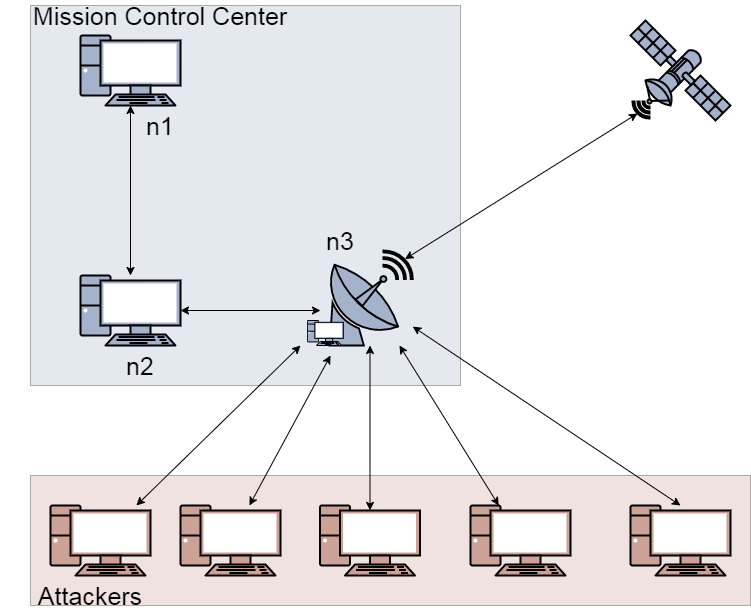
\includegraphics[width=0.5\textwidth]{ddos}
\caption{Netzwerktopologie des DDoS Szenarios}
\end{figure}
Das Grundprinzip des Angriffes ist dem im vorherigen Szenario Verwendeten sehr ähnlich. Hier wird jedoch \textit{n3} deutlich stärker ausgelastet, da nicht nur ein Angreifer Bundles sendet, sondern fünf. \par
Tatsächlich ist die Belastung so hoch, dass \textit{n3} wenige Sekunden nach Start des Angriffes kaum noch Bundles annehmen kann. Es kommt also zu einer Ansammlung von Bundles auf den Angreiferknoten, welche ihre Bundles nicht mehr schnell genug an \textit{n3} senden können. Ansonsten ist das Ergebnis das Gleiche wie im Bundle Flooding Szenario, wobei der Verbindungsabbruch durch das höhere Bundleaufkommen  hier etwas eher auftritt.

\subsection{Config Take Over}
Dieses Szenario simuliert einen Angriff auf die Konfigurationsdaten eines kompromittierten Knotens. Die bei dem Szenario verwendete Netzwerktopologie besteht aus einem Angreifer außerhalb des ION-Netzwerks und zwei Knoten innerhalb des Netzwerks, wobei einer davon kompromittiert ist.
\par
\begin{figure}[h]
\centering
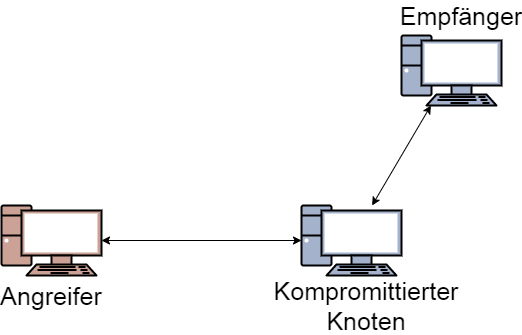
\includegraphics[width=0.5\textwidth]{cto}
\caption{Netzwerktopologie des Config Take Over Szenarios}
\end{figure}
Das Ziel des Angriffs ist es den \textit{kompromittierten Knoten} so zu Sabotieren, dass dieser keine Bundles mehr verschickt und die von ihm ausgehenden Bundles sich bei ihm stauen.
Dafür muss der eine \textit{Knoten} durch einen Phishing-Angriff oder einem ähnlichen so manipuliert sein, dass dadurch im Hintergrund nun \texttt{ncat} ausgeführt wird. \texttt{ncat} liest dabei die Daten, die auf einem spezifischen Port bei dem Knoten ankommen und piped sie dann in einen Bash-Befehl.
Der \textit{Angreifer} sendet über \texttt{ncat} nun ein Skript, welches die Konfiguraionsdaten von ION bzw. vom Bundle Protocol so ändert, dass der Knoten über das Bundle Protocol nicht mehr auf die Transportprotokolle zugreifen kann. Dadurch stauen sich die Bundles beim Bundleausgang auf dem angegriffenen Knoten.
Nach 10 Sekunden gibt das Skript über einen erneuten Eingriff in die Konfigurationsdateien von ION bzw. BP die Transportprotokolle wieder frei, sodass die gestauten Bundles nun ankommen.
Um das Szenario zu visualisieren, wird das Skript \texttt{othervis.sh} im spezifischen Ordner des Szenarios benutzt.

\subsection{Config Take Over Satellite}
Dieses Szenario simuliert einen Angriff auf die Konfigurationsdaten eines \textit{Satelliten} über einen \textit{kompromittierten Knoten}. Die bei dem Szenario verwendete Netzwerktopologie besteht aus einem \textit{Angreifer} außerhalb des ION-Netzwerks und ansonsten dem gleichen Aufbau wie beim Bundle Flooding Szenario, nur dass die Verbindung zum \textit{Satelliten} stabil ist, also nicht alle 30 Sekunden unterbrochen wird und dass der Knoten \textit{n3} kompromittiert ist.
\par
\begin{figure}[h]
\centering
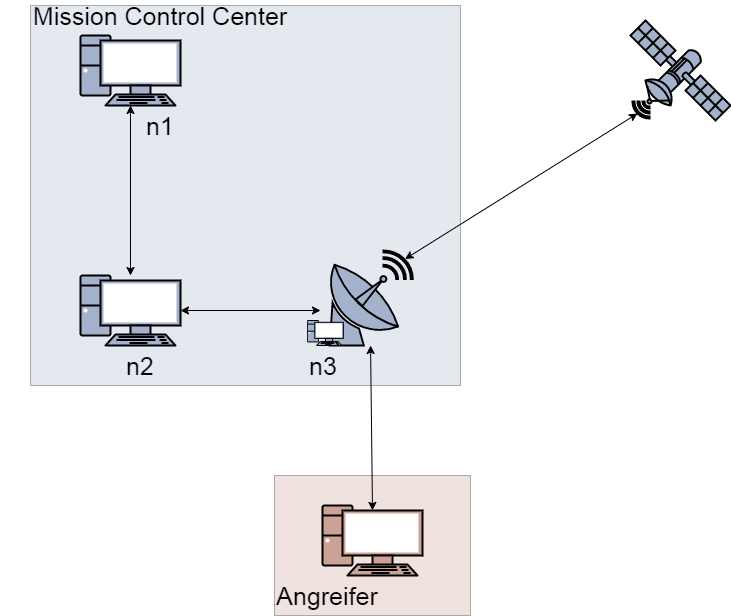
\includegraphics[width=0.5\textwidth]{ctos}
\caption{Netzwerktopologie des Config Take Over Satellite Szenarios}
\end{figure}
Das Ziel des Angriffs ist es, über den kompromittierten Knoten den \textit{Sateliten} lahmzulegen.
Dabei ist der Knoten \textit{n3} wieder so manipuliert, dass auf diesem im Hintergrund \texttt{ncat} läuft. Dazu wird auch angenommen, dass auf dem \textit{Satelliten} ein Tool namens \texttt{lgagent} läuft, womit der \textit{Satellit} seine Kontaktdaten (Wann ist welcher Knoten erreichbar) aktuell halten kann.
Der \textit{Angreifer} sendet nun über ncat ein Skript, welches auf dem Knoten \textit{n3} ein Tool namens \texttt{lgsend} ausführt. \texttt{lgsend} sendet nun über das Bundle Protocol ein Commandfile an den \textit{Satelliten}, welches der \texttt{lgagent} ohne irgendwelche Sicherheitsüberprüfungen direkt ausführt, wodurch der \textit{Satellit} offline geht.
Das Szenario wird visualisiert über das Skript \texttt{othervis.sh} und die beiden Skripte, die auch beim Bundle Flooding Szenario im Einsatz sind.

\subsection{Slowloris}
Im Gegensatz zu den bisher diskutierten Szenarios benötigen Application Layer Denial of Service Angriffe kein bereits kompromittiertes System, um zu funktionieren. Das in diesem Abschnitt näher betrachtete Szenario setzt dabei einen Slowloris Angriff erfolgreich um. Wir nutzen in dem Szenario \texttt{slowloris.py} (Version 0.2.2; Yaltirakli, G., 2015)\cite{gkbrkslowloris}, ein Python Skript, welches die Attacke auf das Zielsystem ausführt.\par
Die hier simulierte Situation ist ein Angriff auf ein Katastrophenfrühwarnsystem. Die Netzwerktopologie ist die Folgende:
\begin{itemize}
\item eine Messstation
\item ein Satellit für die Datenübermittlung
\item ein Kontrollzentrum
\item ein Emergency Broadcast System
\item ein Angreifer, der die Verbindung zwischen Messstation und Satellit stört
\end{itemize}
Dabei sind die Systeme des Frühwarnsystems in Reihe geschaltet und zusätzlich der Angreifer mit dem Satelliten verbunden. Als Transportprotokoll kommt TCP zum Einsatz.
Wie auch in den vorherigen Szenarien werden die einzelnen Knoten durch CORE Routerknoten emuliert.\par
\begin{figure}[h]
\centering
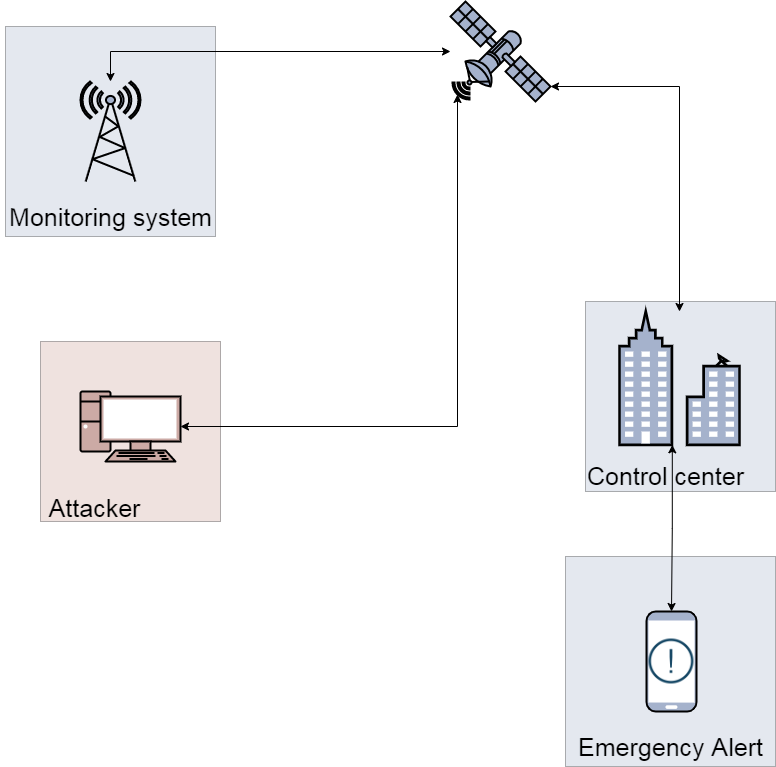
\includegraphics[width=0.5\textwidth]{slowloris}
\caption{Netzwerktopologie des Slowloris Szenarios}
\end{figure}
Das Ziel des Denial of Service Angriffs ist das Lahmlegen des Zielsystems unter minimaler Verwendung von Netzwerkressourcen. Dies wird erreicht, indem das Angreifersystem möglichst viele Verbindungen zum Zielsystem aufbaut und diese so lange wie möglich offenhält.\par
In diesem Szenario wird dieser Effekt durch das Ausführen von dem \texttt{slowloris.py} Skript auf dem Knoten, der den Angreifer simuliert, erreicht. Das Skript baut so viele Verbindungen wie möglich zu dem Satelliten auf und versendet nur Teilanfragen. Dies hat den Effekt, dass auf dem Satelliten die Anfragen nie vollständig abgeschlossen werden und die Verbindungen zum Angreifer bestehen bleiben. Werden auf diese Weise genügend Verbindungen gleichzeitig blockiert, so kann der Satellit von der Messstation eingehende Verbindungsanfragen nicht annehmen und die Verbindung zwischen Messstation und Kontrollzentrum ist unterbrochen. Die Verbindungsunterbrechung tritt bereits den Bruchteil einer Sekunde nachdem der Angriff gestartet wurde, auf und ist somit deutlich schneller als bei dem Bundle Flooding Angriff.\par
Diese Art Denial of Service Attacke zeichnet sich besonders dadurch aus, dass sie vollkommen vom ION-Netzwerk unabhängig ist, also kein bereits kompromittiertes System innerhalb des Netzwerkes benötigt wird, um erfolgreich die Verbindung zu stören. Ein Angreifer mit ausreichend leistungsstarker Hardware könnte damit sehr einfach sämtlichen Traffic in kritischen Systemen zum Erliegen bringen, sofern diese TCP als Transportprotokoll nutzen.\par
Die Visualisierung der Auswirkungen des Angriffes in unserer Netzwerksimulation erfolgt wieder durch ein Shell-Skript, welches das Ergebnis des Pings von Messstation zum Kontrollzentrum in einer Konsole ausgibt.

\section{Erweiterung}
Wir haben bei der Planung und Entwicklung dieses Tools Wert darauf gelegt, dass schnell und einfach neue Szenarien integriert werden können. Diese neu angelegten Szenarien liegen standardmäßig unter /home/User/.core/configs/ion/. Dies ist auch der Pfad, der von dem Start-Skript untersucht wird, um die verfügbaren Szenarien anzuzeigen. Er wird im Folgenden als 'Basispfad' bezeichnet.\par


\subsection{Aufbau eines virtuellen Netzwerks mit CORE}
\subsubsection{Start des Common Open Research Emulator}
CORE (Common Open Research Emulator) ist ein Tool, mit welchem man leicht virtuelle Netzwerke aufbauen kann. Als Emulator baut CORE eine Repräsentation eines in Echtzeit laufenden realen Computernetzwerks auf, anstelle einer Simulation, bei der abstrakte Modelle verwendet würden. Diese Emulation kann, bei Bedarf auch mit physischen Netzwerken und Routern verbunden werden und bietet eine Umgebung, um echte Applikationen und Protokolle zu testen.\cite{core-docs} \par
Zum Betrieb von CORE ist es wichtig, dass der \texttt{core-daemon} im Hintergrund läuft. Der Status des Daemons lässt sich mittels \texttt{sudo service core-daemon status} abfragen. Sollte der Daemon nicht gestartet sein, muss \texttt{sudo service core-daemon start} ausgeführt werden. Nun kann man mittels \texttt{core-gui} die graphische Oberfläche von CORE starten. In der folgenden Abbildung ist der Ablauf veranschaulicht.\par
\begin{figure}[ht]
\centering
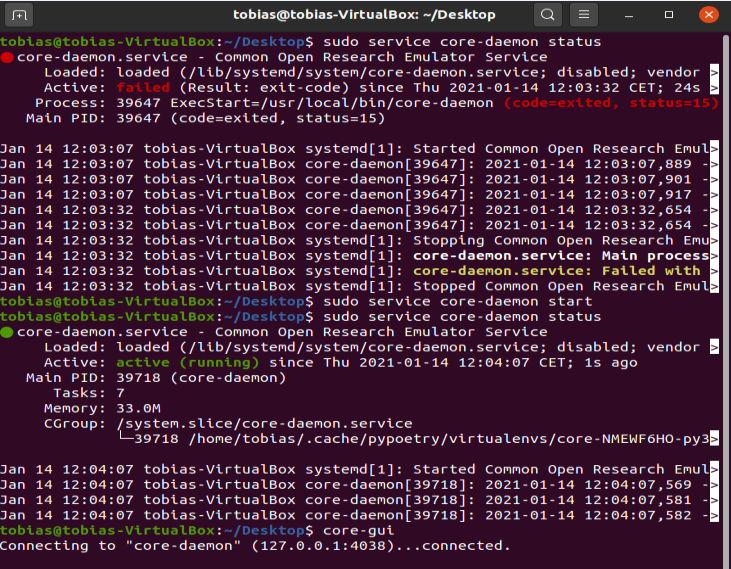
\includegraphics[width=0.7\textwidth]{core-start}
\caption{Start der CORE-Oberfläche}
\end{figure}
Das User Interface von CORE zu erklären würde im Rahmen dieses Dokuments zu weit führen, allerdings gibt es eine ausführliche englische Dokumentation zu den einzelnen Knotentypen, dem User Interface und vielen weiteren Themen direkt von CORE. Diese ist unter dem folgenden Link zu finden: \url{https://coreemu.github.io/core/}\par
Das Anlegen eines neuen CORE-Projekts sollte direkt in einem neuen Ordner im Basispfad erfolgen, um später Probleme zu vermeiden. Dabei ist wichtig, das der Name der <Szenario>.imn Datei d\par

\subsubsection{Aufbau eines Netzwerks mit CORE}
Die Netzwerke in unseren Szenarien bestehen der Einfachheit halber ausschließlich aus Knoten vom Typ Router, welche durch physische Links verbunden sind. Das Verwenden von anderen Knotentypen und Wireless LAN ist natürlich möglich, aber nicht von uns getestet.\par
Wireless LAN in CORE unterstützt sogenanntes Mobility Scripting, wodurch sich Knoten zur Laufzeit aus der Verbindungsreichweite entfernen können, um Verbindungsabbrüche zu erzwingen. Diese Verbindungsabbrüche in CORE haben \textbf{keine} Auswirkung auf die Verbindung der ION Nodes. Man muss durch Anpassen der ION-Konfigurationsdateien zur gleichen Zeit für einen Verbindungsstopp sorgen.

\subsubsection{Integration von ION}
Die Integration von ION in CORE erfolgt in drei einfachen Schritten, die auf jedem Knoten ausgeführt werden müssen.
\begin{itemize}
\item Einrichten eines UserDefined-Services zum Ausführen eines Setup-Skripts
\item Zuweisen der von ION benötigen Verzeichnisse
\item Anlegen des Setup-Skripts
\end{itemize}\par
Zunächst muss ein Service eingerichtet werden, der ein Setup-Skript ausführt, welches dann ION auf dem Knoten startet. Diesen legt man wie folgt an: Doppelklick auf den Knoten $\rightarrow$ Services $\rightarrow$ UserDefined. Im Tab 'Files' den file name \texttt{'setup.sh'} (ohne '') eingeben und auf den Button neben der Eingabeleiste klicken. 'Use text below for file contents' auswählen und in die Box darunter das folgende Skript kopieren.
\begin{verbatim}
    dirn=`dirname $SESSION_FILENAME`
    sh $dirn/nodeSetup.sh
\end{verbatim}
Die Backticks um "dirname [...]" können evtl. nicht richtig aus diesem Dokument kopiert werden und müssen dann manuell gesetzt werden.\par
Als nächstes müssen die Verzeichnisse zugewiesen werden. Dazu auf den Tab 'Directories' wechseln, unten rechts auf den 'Verzeichnis hinzufügen' Button (
\includegraphics[height=\fontcharht\font`\B]{new}) klicken und /var/ion hinzufügen.\par
Zuletzt muss dem Knoten noch mitgeteilt werden, dass das in Schritt 1 angelegte \texttt{'setup.sh'} Skript ausgeführt werden soll. Dies geschieht im 'Startup/Shutdown' Tab. In die Zeile unter 'Startup commands' \texttt{'sh setup.sh'} schreiben und auf den 'Hinzufügen' Button (
\includegraphics[height=\fontcharht\font`\B]{new}) klicken. Danach kann man die Einstellungen durch Klick auf 'Apply' anwenden und der Knoten ist konfiguriert. Danach muss das CORE-Projekt noch einmal gespeichert werden, da sonst die konfigurierten Knoten bei Neustart verloren gehen.\par
Bach dem Speichern kann man das CORE-GUI erst einmal schließen.

\subsubsection{nodeSetup.sh}
Das Skript \texttt{nodeSetup.sh} wird von CORE ausgeführt, sobald ein Knoten gestartet wurde und sorgt dafür, dass auf dem Knoten ION läuft. Es muss immer im gleichen Verzeichnis liegen wie die \texttt{<Szenario>}.imn Datei. Für die genaue Verzeichnisstruktur siehe \textbf{\ref{svz}}.\par
Wir empfehlen ein schon vorhandenes \texttt{nodeSetup.sh} Skript aus einem Szenario-Ordner zu kopieren und zu modifizieren. Der Teil, in dem verschiedene ION-Services gestartet werden, ist die if-else-Abfrage nach
\begin{verbatim} 
    ionstart -I n\$IPN\_NODE\_NUMBER.rc >> \$LOG
\end{verbatim}
Sollte zudem eine Visualisierung der Anzahl von Bundles auf jedem Knoten gewünscht sein, muss sichergestellt werden, dass unter der if-else-Abfrage die Zeile \begin{verbatim}
    sh bundlecount.sh "$IPN_NODE_NUMBER"
\end{verbatim} und unter \begin{verbatim}
    cp $BASE_DIR/n$IPN_NODE_NUMBER/* .
\end{verbatim} die Zeile 
\begin{verbatim}
    cp $BASE_DIR/bundlecount.sh .
\end{verbatim} eingefügt wurden. Mehr dazu im Abschnitt \textbf{\ref{visualisierung}}.

\subsection{Konfiguration von ION}
Es ist wichtig, dass für jeden Knoten, der in CORE definiert wurde, ein eigener Ordner im Szenarioverzeichnis angelegt wird. In diesen Ordnern befinden sich die ION-Konfigurationsdateien der einzelnen Knoten (vgl. \textbf{\ref{svz}}).\par
Die Konfigurationsdateien, die ION nutzt um die Nodes zu initialisieren, sind komplex genug, um dazu eine eigene Dokumentation zu schreiben. Eine grobe Übersicht liefert der ION Deployment Guide im ion-open-source-4.0.0 Ordner (Anwendungsverzeichnis, siehe \textbf{\ref{avz}}, der sich im dtn-dos Verzeichnis befindet. Außerdem gibt es eine Serie an Videos auf YouTube, welche sich mit ION befasst. Das die Konfiguration behandelnde Video kann man unter folgendem Link finden: \url{https://www.youtube.com/watch?v=gEMoxbUz-jo}. In diesem Video wird nicht erklärt, dass man die einzelnen Konfigurationsdateien auch in einer Datei zusammenfassen kann. Deshalb lohnt es sich auch, zusätzlich die Konfigurationsdateien in unseren Szenarien anzusehen.  

\subsection{Visualisierung des Szenarios}\label{visualisierung}
Jedes Szenario hat unterschiedliche Anforderungen an die Visualisierung. Für unsere Szenarien haben wir drei Visualisierungen entwickelt. Diese  müssen auf der obersten Ebene des Szenarioverzeichnisses liegen und werden durch das start\_dtndos.sh-Skript, beziehungsweise das nodeSetup.sh Skript (gilt nur für bundlecount.sh), gestartet.

\subsubsection{bundlecount.sh und bundlewatch.sh}
Die beiden Skripte \texttt{bundlecount.sh} und \texttt{bundlewatch.sh}, zeigen die Anzahl an Bundles auf jeder Node an. Dabei wird \texttt{bundlecount.sh} auf allen Nodes im Hintergrund ausgeführt und schreibt pro Sekunde einmal die Anzahl der auf der Node gespeicherten Bundles in eine Logdatei, die dann von \texttt{bundlewatch.sh} ausgelesen und in einem Terminal-Fenster visuell aufbereitet wird.\par
Damit diese Visualisierung funktioniert, müssen die beiden Skripte im Verzeichnis des Szenarios liegen. Desweiteren muss auf jedem Knoten, durch das \texttt{nodeSetup.sh} Skript, das \texttt{bundlecount.sh} gestartet werden.

\subsubsection{pingvis.sh}
Dieses Skript wird vom \texttt{start\_dtndos.sh} Skript ausgeführt, um zu verfolgen, wann die Verbindung zwischen zwei Nodes abbricht. Dazu wird die Ausgabe des Bundle Pings auf einer Node in ein Logfile umgeleitet, welches vom pingvis Skript dann in einem Terminal ausgegeben wird.\par
Auf den Nodes sind standardmäßig die Watch Characters von ION aktiviert. Dies zeigt sich in der Ausgabe des Skriptes. Jedes Mal, wenn ein Bundle losgeschickt wird, wird einmal das Zeichen 'a' ausgegeben. Bestätigt die angepingte Node den Eingang des Signals, so wird außerdem die Response mit Round-Trip-Time ausgegeben. Gibt es einen Verbindungsabbruch, erkennt man dies an dem Fehlen ebendieser Antwort auf die gesendeten Bundles. Im Terminal tauchen dann nur noch die 'a's für gesendete Anfragen auf. 

\subsubsection{othervis.sh}
Das \texttt{othervis.sh} Skript ist für alle weiteren szenariospezifischen Visualisierungen gedacht. Es wird zum Beispiel im Slowloris-Szenario genutzt, um anzuzeigen, wann genau der Angriff startet. Durch die Anpassung auf ein bestimmtes Szenario, kann man othervis.sh-Skripte aus anderen Szenarien nur bedingt kopieren und wiederverwenden.

\section{Fazit und Ausblick}
Zusammengefasst lässt sich sagen, dass es uns gelungen ist, alle gestellten Anforderungen zu erfüllen. Das Ergebnis ist eine vollständige, leicht erweiterbare Testsuite zum Untersuchen der Auswirkungen von Denial of Service-Angriffen auf die ION-DTN-Implementierung. Diese Dokumentation markiert den Release der Version 1.0 von dtn-dos.\par
Einige Features wurden von uns als interessant empfunden, haben es aber nicht in diese Version von dtn-dos geschafft. Diese sind im Folgenden aufgelistet:
\begin{itemize}
    \item Detaillierte Statistiken nach Ende eines Szenarios
    \item Szenarien zur Simulation weiterer verbreiteter DoS-Angriffsarten
    \item Graphische Liveauswertung des Netzwerkverkehrs während der Ausführung
    \item Test, ob andere DTN-Implementationen integriert werden können
\end{itemize}


\newpage
\printbibliography
\end{document}